%% Direttive TeXworks:
% !TeX root = ../semprini_luca_tesi.tex
% !TEX encoding = UTF-8 Unicode
% !TEX program = arara
% !TEX TS-program = arara
% !TeX spellcheck = it-IT

%% Direttive Arara:
% arara: pdflatex: { shell: yes, synctex: yes, action: batchmode, options: "-halt-on-error -file-line-error-style" }
% arara: frontespizio
% arara: biber
% arara: pdflatex: { shell: yes, synctex: yes, action: batchmode, options: "-halt-on-error -file-line-error-style" }
% arara: pdflatex: { shell: yes, synctex: yes, action: nonstopmode, options: "-halt-on-error -file-line-error-style" }
\chapter{Analisi Conclusiva}


\section{Situazione Attuale}
Allo stato attuale, il linguaggio Kotlin è in continua evoluzione. Per quanto riguarda l'ambito della piattaforma Android, fin dalle primissime release, Kotlin ha sempre avuto un appeal particolare nei confronti di molti sviluppatori: essendo stato progettato per rendere la progettazione di applicazioni più "divertente" rispetto all'utilizzo di Java, ha da subito riscosso un grande interesse nella community Java, ma non solo. Molte aziende e sviluppatori indipendenti hanno immediatamente optato per iniziare uno switch a livello di codice sorgente da Java a Kotlin, in quanto particolarmente attratti dalla filosofia e dalle funzionalità del linguaggio; tuttavia questa operazione ha rappresentato, a priori, un rischio, poiché il linguaggio era ancora molto giovane e soprattutto non supportato dal team di Google. Successivamente alla Google I / O del 17 maggio 2017, l'assunzione di Kotlin da parte di moltissime aziende come linguaggio principale in cui sviluppare le proprie applicazioni mobile ha subito un’impennata notevole, guidata dall’entusiasmo che ha contaminato gli sviluppatori Android a seguito dell'annuncio ufficiale alla conferenza.\\

Attualmente, ci sono moltissime aziende note che lo utilizzano in produzione: ad esempio, Pinterest è stata una delle prime compagnie a farne uso in maniera preponderante per la sua app Android. Un altro grande esempio è rappresentato dalla situazione di Basecamp: la compagnia americana fa già uso di Kotlin nel 100\% del codice sorgente della propria applicazione. Per mostrare altri esempi di aziende che si stanno affidando a Kotlin in questo ambito, si possono citare Trello, Netflix, Prezi, Hootsuite, NBC News Digital, e molte altre.\\

Un altro importante fatto da riportare riguarda le offerte di lavoro da parte di molte aziende: queste ultime stanno iniziando a richiedere competenze approfondite di linguaggio Kotlin per i loro posti di lavoro. Non solo, molte compagnie stanno iniziando a fare investimenti di denaro nella formazione dei propri dipendenti in modo da avere sviluppatori Kotlin.\\
Quindi, anche se Kotlin non è adottato nella maggior parte delle aziende per progettare applicazioni Android, vi sono già alcune compagnie che ne stanno facendo uso, le quali, durante la propria crescita, avranno sempre più bisogno di esperti di Kotlin. Molti sviluppatori indipendenti che avevano scommesso su un linguaggio appena annunciato come era Kotlin agli inizi, approfondendone e apprendendone le funzionalità più avanzate, hanno oggi facilmente trovato lavoro grazie a questa intuizione.\\

Inoltre, Kotlin risulta molto facile da imparare, sia per le sue caratteristiche sintattiche (che ricordano quelle di molti linguaggi esistenti e familiari per gli sviluppatori di applicazioni mobili, come Java, JavaScript e Groovy), sia per i tool di supporto all'apprendimento, come {\bfseries Kotlin-koans} \cite{kotlinKoans}: un set di esercizi per familiarizzare il programmatore con la sintassi di Kotlin. Ogni esercizio viene creato come uno Unit-test che fallisce di default, e il compito dello "studente" è quello di modificare alcune parti di codice per permettere che il test abbia successo. È possibile utilizzare Koans online, direttamente all'interno di IntelliJ IDEA o Android Studio, o clonando il progetto da GitHub. Un altro tool molto utile in questo senso è il già citato convertitore "Java-to-Kotlin" e "Kotlin-to-Java", che permette al programmatore di iniziare a scrivere codice Kotlin a piccoli passi, inizialmente traducendo il proprio codice Java automaticamente in Kotlin, per imparare meglio la sintassi.\\
Sotto l'aspetto istruttivo, il team di Kotlin suggerisce anche numerose letture utili per familiarizzare con il linguaggio, come
Kotlin in Action \cite{kaction}, Kotlin for Android Developers \cite{leiva}, Programming Kotlin \cite{programmingKotlin} e altri.\\

Ad oggi, successivamente alla KotlinConf e dopo quasi 7 mesi dall'annuncio ufficiale di Kotlin come linguaggio first-class per Android al Google I / O, il numero di app sul Google Play Store implementate in Kotlin è più che raddoppiato: attualmente, oltre il 17\% dei progetti in Android Studio 3.0 utilizza Kotlin \cite{ktUpdateAndroidDevBlog}, e la tendenza è in continuo aumento. Per considerare l'importanza dell'annuncio da parte di Google di supportare Kotlin come linguaggio first-class, si noti la figura \ref{GoogleInterest}.\\
\\
\\

\begin{figure}[ht]
  \centering
  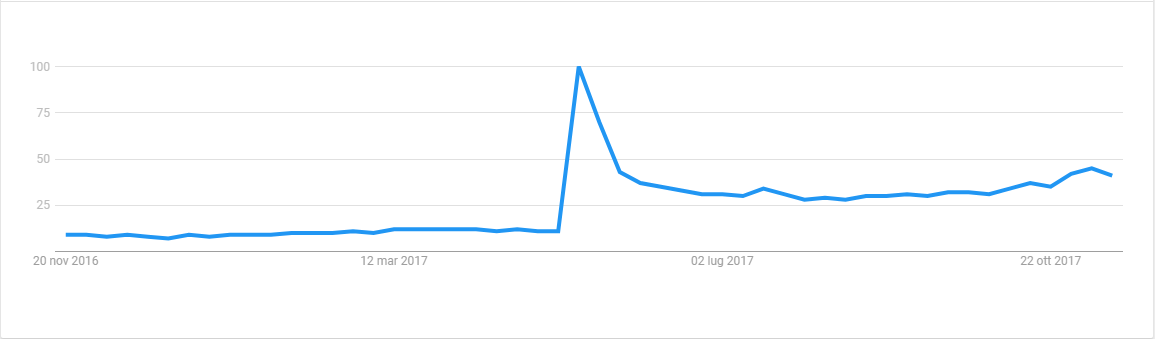
\includegraphics[scale=0.5]{GoogleInterest.png}
  \caption{{\bfseries Interesse nel tempo per Kotlin stimato da Google Trends}}
  \label{GoogleInterest}
\end{figure}

Come si può notare, l'impennata della curva di interesse riportata nel grafico corrisponde esattamente con l'annuncio del 17 maggio 2017; l'interesse va successivamente calando, fino ad assestarsi su un valore comunque di molto superiore a quello che possedeva prima del Google I / O, ma risulta comunque in continua ascesa. Anche le date del 3 e 4 novembre 2017 contribuiscono al grafico: la leggera risalita che si può notare sulla parte destra del grafico, infatti, corrisponde proprio alla KotlinConf di San Francisco.

\section{Prospettive future per Kotlin}

Secondo un rapporto \cite{realmReport} pubblicato da Realm \cite{realm} (un famoso fornitore di un popolare e indipendente database mobile in-app) pubblicato il 25 settembre 2017, la tendenza all'adozione di Kotlin è aumentata molto rapidamente e potrebbe superare Java nel dicembre del 2018, ovvero circa 17 mesi dopo che Google ha annunciato il supporto ufficiale al linguaggio di JetBrains e 2 anni e mezzo dopo che Kotlin ha raggiunto la v1.0; per fare un confronto, per quanto riguarda il sistema iOS, ci sono voluti solo 14 mesi dopo il rilascio di Swift v1.0 prima di raggiungere lo stesso picco rispetto ad Objective-C, ma ovviamente si è trattato di una situazione molto diversa: Swift è, infatti, un linguaggio proprietario di Apple, pensato esclusivamente per sviluppare applicazioni iOS.\\

I risultati del rapporto si basano su un'analisi del comportamento di oltre 100.000 sviluppatori che utilizzano il database di Realm nelle loro applicazioni. Il DB mobile è attualmente installato su oltre 3,5 miliardi di applicazioni iOS e Android, tra cui Starbucks, SAP, eBay, Intel e Alibaba. Il rapporto è il primo di una serie trimestrale pianificata, ha spiegato Paul Kopacki, VP del marketing di Realm.\\
La società ha compilato i dati sullo sviluppo di applicazioni mobili che utilizzano il loro database da agosto 2015 e questa prima edizione del Realm Report si è concentrata sui linguaggi di programmazione più popolari che gli sviluppatori utilizzano per creare applicazioni mobili e ha riscontrato quanto segue.\\

\begin{figure}[ht]
  \centering
  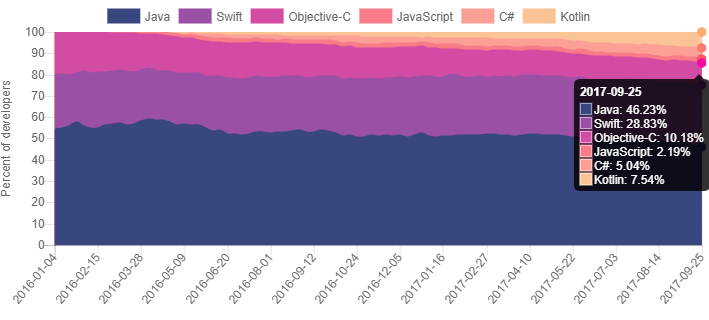
\includegraphics[scale=0.60]{languages.png}
  \caption{{\bfseries Linguaggi di programmazione per sistemi mobile più popolari secondo Realm}}
  \label{languages}
\end{figure}

Come si può notare dalla tendenza mostrata dal grafico in figura \ref{languages}, Java sta perdendo il mindshare (appetibilità) degli sviluppatori ed anche velocemente: la percentuale di applicazioni Android create utilizzando Java è diminuita del 6.1\% e negli ultimi quattro mesi è scesa dal 50.7\% al 46.2\% delle app complessive, e questo significa che l'adozione di Kotlin come principale linguaggio con cui programmare applicazioni Android sta esplodendo: il numero di applicazioni create utilizzando Kotlin, infatti, è cresciuto del 125\%. Un altro dato interessante fornito da questo rapporto riguarda applicazioni già esistenti scritte in Java: il 20\% delle applicazioni Kotlin costruite dopo la conferenza Google I / O erano state precedentemente costruite con Java, il che significa che non c'è stata solo un'esplosione del linguaggio per quanto riguarda i nuovi progetti, ma che si sta operando uno switch di linguaggio di programmazione anche nelle applicazioni già consolidate ed inizialmente progettate in Java.\\
Nonostante il supporto a Java 8 dalla versione 3.0 di Android Studio, gli sviluppatori stanno mostrando sempre più interesse per il nuovo linguaggio proposto da JetBrains. Di seguito si riporta un grafico reso disponibile da Realm, che fotografa la situazione di Kotlin e Java in due momenti ravvicinati, ma molto differenti.\\

\begin{figure}[ht]
  \centering
  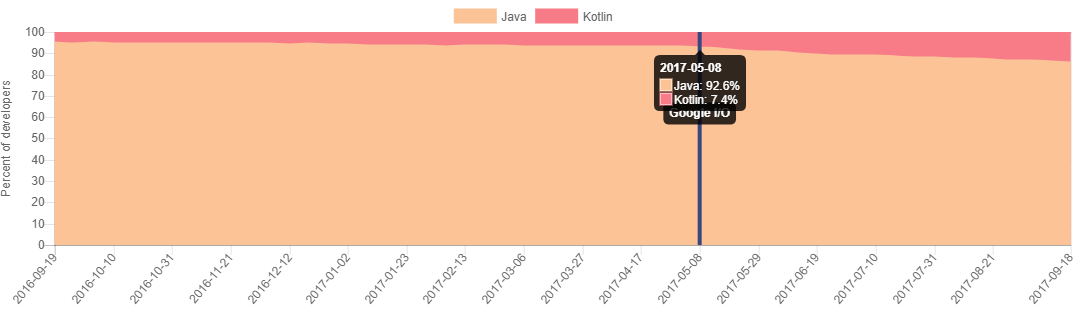
\includegraphics[scale=0.4]{downloadGIO.png}
  \caption{{\bfseries Utilizo di Kotlin e Java in applicazioni Android prima del Google I / O}}
  \label{gio}
\end{figure}

\begin{figure}[ht]
  \centering
  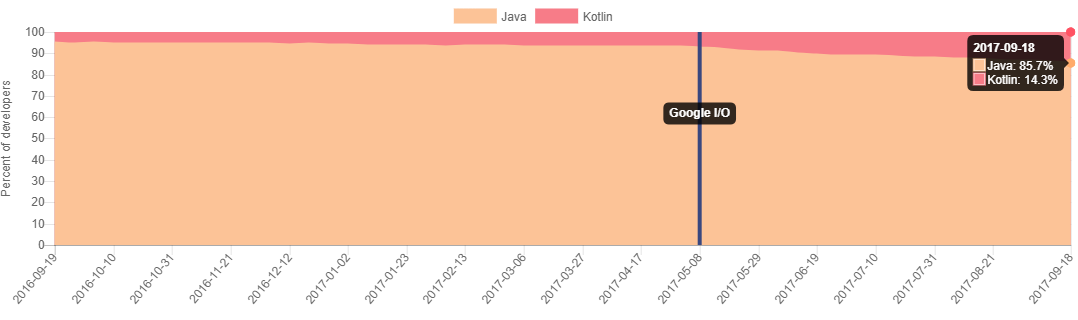
\includegraphics[scale=0.4]{downloadNow.png}
  \caption{{\bfseries Utilizo di Kotlin e Java in applicazioni Android in data 18 settembre 2017}}
  \label{now}
\end{figure}

La figura \ref{gio} riporta i dati dell'utilizzo di Java e Kotlin da parte degli sviluppatori in data 8 maggio 2017, quindi pochi giorni prima dell'annuncio del supporto ufficiale di Google; la figura \ref{now}, invece, mostra quanto velocemente sia accresciuto l'interesse verso il nuovo linguaggio da parte dei programmatori in pochi mesi: dal 7.4\% di utilizzo è, infatti, passato al 14.3\%.\\

Per quanto riguarda le proiezioni future, il rapporto di Realm prevede, come anticipato, che Kotlin supererà Java molto presto. Sulla base dei dati, questo avverrà circa nel mese di dicembre 2018. Realm è abbastanza ottimista sul futuro di Kotlin e non solo, il rapporto afferma, infatti, che "presto, gli sviluppatori Android che non hanno competenze di Kotlin rischieranno di essere considerati come dinosauri" \cite{realmReport}.\\
Ciò significa che gli sviluppatori (quantomeno in ambito Android) che rimarranno ancorati sul linguaggio Java correranno il rischio di diventare obsoleti, per cui le possibilità di trovare un lavoro come programmatori di applicazioni Android saranno ridotte poiché sarà necessaria la conoscenza di un linguaggio più moderno tra i requisiti. Inoltre, Realm prevede un grande futuro per Kotlin anche in altri ambienti come quello server, dove, anche qui, potrebbe arrivare a sostituire Java; con gli ultimi annunci da parte di JetBrains, infine, sta cominciando sempre più a farsi strada la possibilità di un utilizzo di Kotlin su progetti multi-piattaforma, quindi anche su sistemi iOS e servizi web front-end.
Si noti, dunque, un ulteriore grafico reso disponibile da Realm, che riporta, sulla base di una proiezione statistica, la aspettativa di crescita di utilizzo del linguaggio Kotlin nei sistemi Android nei prossimi mesi.\\

\begin{figure}[ht]
  \centering
  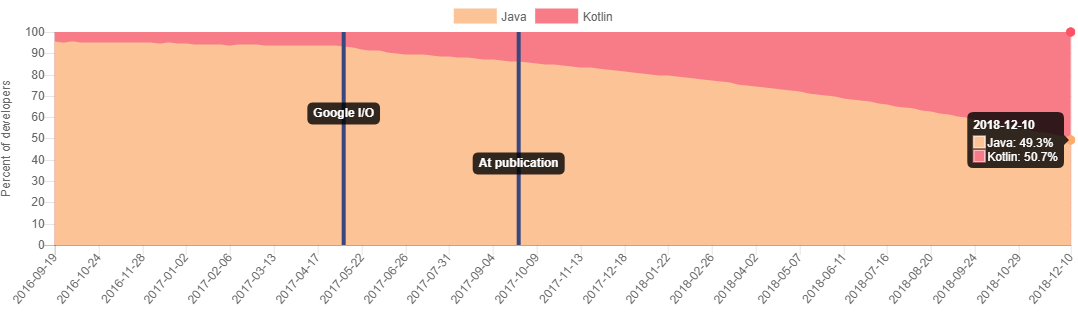
\includegraphics[scale=0.4]{downloadProjected.png}
  \caption{{\bfseries Proiezione del grafico precedente per l'utilizzo di Kotlin rispetto a Java in applicazioni per la piattaforma Android}}
  \label{projected}
\end{figure}

Il grafico in figura \ref{projected} mostra come, sulla base dei dati riportati da Realm e su una proiezione statistica, Kotlin potrebbe soppiantare Java in termini di percentuale di utilizzatori in poco più di un anno dalla pubblicazione del primo rapporto (data contrassegnata dalla linea verticale con etichetta "At publication"). Ovviamente si tratta di una proiezione ottimistica, che prevede che l'entusiasmo dei programmatori nei confronti del nuovo linguaggio cresca con lo stesso andamento con cui è cresciuto nelle settimane immediatamente successive al Google I / O. Tuttavia, non è una proiezione inverosimile, in quanto l'appetibilità di Kotlin agli occhi degli sviluppatori è sicuramente un dato di fatto, e la popolarità del linguaggio sta inesorabilmente crescendo. Infine, il Realm Report non è il solo recente rapporto del settore a notare un aumento della popolarità di Kotlin: Redmonk, Tiobe e RebelLabs hanno riconosciuto il suo impatto, specialmente su Java, che era una volta l'unico linguaggio disponibile per gli sviluppatori Android.
